\subsection{Performance optimizations}
\label{sec:dssmr-optm}

In this section, we introduce two optimizations for \dssmr{}: caching and load
balancing.

\textbf{Caching.} In Algorithm~\ref{alg:client_proxy}, for every command issued
by the client, the proxy consults the oracle. If every command passes by the
oracle, the system is unlikely to scale, as the oracle is prone to becoming a
bottleneck. To provide a scalable solution, each client proxy has a local cache
of the partitioning information. Before multicasting an application command $C$
to be executed, the client proxy checks whether the cache has information about
every variable concerned by $C$. If the cache does have such a knowledge, the
oracle is not consulted and the information contained in the cache is used
instead. If the reply to $C$ is $retry$, the oracle is consulted and the
returned prophecy is used to update the client proxy's cache.
Algorithm~\ref{alg:client_proxy} is followed from the second attempt to execute
$C$ on. The cache is a local service that follows an algorithm similar to that
of the oracle, except it responds only to $consult(C)$ commands and, in
situations where the oracle would return $ok$ or $nok$, the cache tells the
client proxy to consult the actual oracle.


Naturally, the cached partitioning information held by the client proxy may be
out of date. On the one hand, this may lead a command to be multicast to the
wrong set of partitions, which will probably incur in the client proxy having to
retry executing the command. For instance, in Figure~\ref{fig:dssmr-retry} the
client has an out-of-date cache, incurring in a new consultation to the oracle
when executing $C_3$. On the other hand, the client proxy may already have to
retry commands, even if the oracle is always consulted first, as shown in
Figure~\ref{fig:dssmr-detail}. If most commands are executed without consulting
the oracle, as in the case of $C_4$ in Figure~\ref{fig:dssmr-retry}, we avoid
turning the oracle into a bottleneck. Moreover, such a cache can be updated
ahead of time, not having to wait for an actual application command to be issued
to only then consult the oracle. This way, the client proxy can keep a cache of
partitioning information of variables that the proxy deems likely to be accessed
in the future.

\textbf{Load balancing}. When moving variables, the client proxies may try to
distribute them in a way that balances the workload among partitions. This way,
the system is more likely to scale throughput with the number of server groups.
One way of balancing load is by having roughly the same number of state
variables in every partition. This can be implemented by having client proxies
choosing randomly the partition that will receive all variables concerned by
each command (at line~\ref                {algline:client:partition} of
Algorithm~\ref{alg:client_proxy}). Besides improving performance, balancing the
load among partitions prevents the system from degenerating into a
single-partition system, with all variables being moved to the same place as
commands are executed.


\begin{figure*}
\begin{minipage}[b]{1\linewidth} % A minipage that covers the whole width of the
page
\centering
      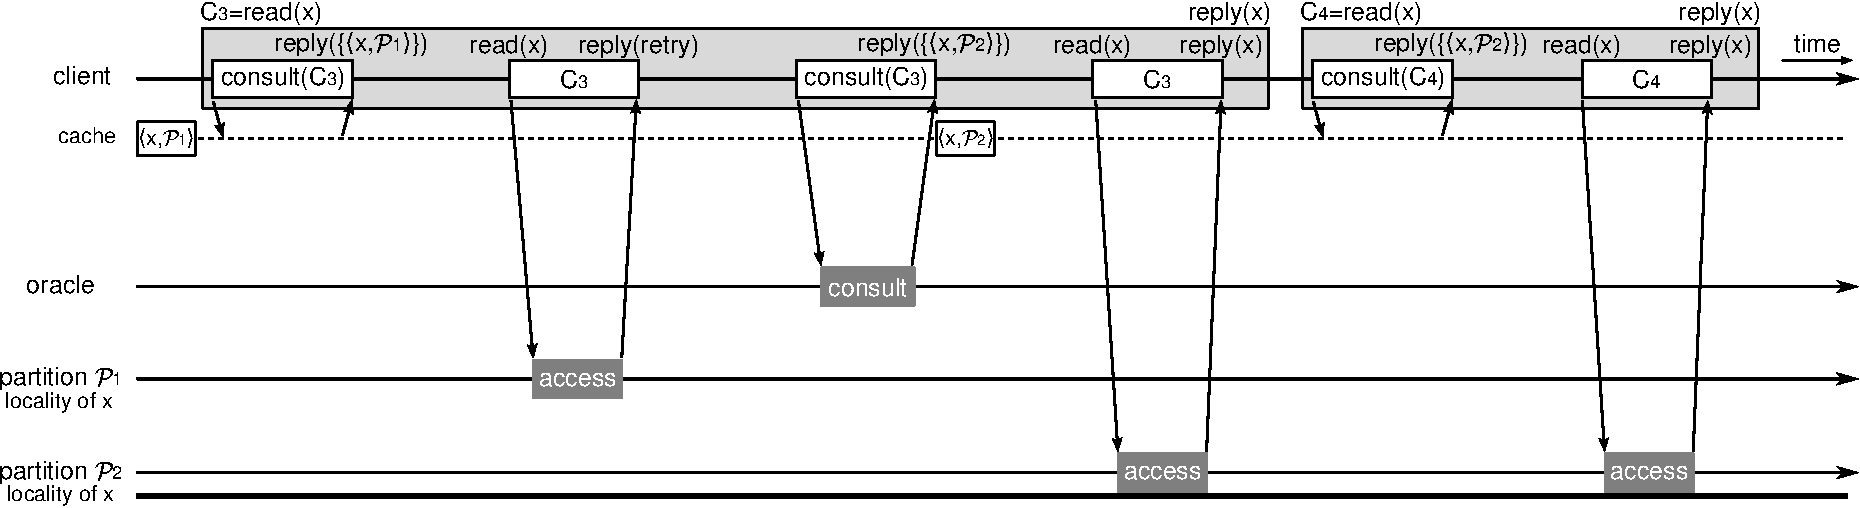
\includegraphics[width=1.0\linewidth]{figures/dssmr-retry}
\end{minipage}
\caption{Each client proxy in \dssmr\ maintains a cache in order to avoid  consulting the oracle. White boxes represent actions of the client proxy.}
\label{fig:dssmr-retry}
\end{figure*}

